\begin{figure*}[!tp]
	\center
	\begin{subfigure}{0.28\linewidth}
		\includegraphics[width=\linewidth]{figs/multi_autoencoder_bler_awgn}
		\caption{AWGN channel}
	\end{subfigure}
	\begin{subfigure}{0.28\linewidth}
		\includegraphics[width=\linewidth]{figs/multi_autoencoder_bler_rician}
		\caption{Rician fading channel}	
	\end{subfigure}
	\begin{subfigure}{0.28\linewidth}
		\includegraphics[width=\linewidth]{figs/multi_autoencoder_bler_rayleigh}
		\caption{Rayleigh fading channel}	
	\end{subfigure}
	\caption{The block error rates (BLERs) of our trained autoencoders compared with simulated results for different numbers of users over a range of SNR values in our multi-user system.}
	\label{fig:multi_autoencoder_bler}
\end{figure*}

\section{Experiments and Evaluation}
\label{s:eval}
Our experiments are divided into two sections. In the first section, we evaluate the performance of our trained autoencoder wireless networks. In the next section, we discuss the performance of our implemented covert models in both single-user and multi-user systems in terms of their robustness to different channel models, data rates, and numbers of users.

\subsection{Baseline Single-User Autoencoder's Performance}
We implemented an autoencoder communication network for normal communication between UserRX and UserTX. An autoencoder \(Autoencoder (n, k)\) is a neural network communication model that sends \(k\) bits of data in \(n\) channel uses. To make our results comparable with the original paper \cite{o2017introduction}, we chose our default parameters to be 8 and 4 for the number of channel uses and binary message size, respectively. However, we also evaluated our models for two other sets of parameters with the same data rate but different numbers of channel uses. This allowed us to examine how increasing the number of channel uses, or channel dimensionality, would affect communication performance. To train our autoencoder model, we generated two datasets for training and testing by randomly generating binary messages \(s\) of size \(k\). Specifically, we used 8192 random binary messages in the training set and 51200 random binary messages in the test set. We created a much larger dataset for testing to ensure that each symbol \(y\) undergoes various channel distortions, providing a more accurate evaluation of the model's performance. We set the learning rate to 0.001 and optimized the model using the Adam optimizer \cite{kingma2014adam}. We used a batch size of 1024 and trained the model for 100 epochs. For the channel configuration, \textbf{we fixed the signal-to-noise ratio (SNR) value during training but evaluated the model's performance over a range of SNRs}. The SNR value for the AWGN channel was set to 4dB, while the values for the Rayleigh and Rician fading channels were 16dB. We chose these SNR values experimentally by training the models on different SNR values and identifying the value on which the model performed best.

Figure \ref{fig:autoencoder_bler} displays the block error rate (BLER) performance of our trained autoencoder communication models for various sets of parameters across a range of SNR values. The models were trained individually on AWGN, Rayleigh, and Rician fading channels and tested on the same channel they were trained on.
The plot reveals that despite having the same data and coding rate, increasing the channel dimension slightly enhances the performance of the autoencoder models. This phenomenon was first identified in \cite{o2017introduction}, which demonstrated that autoencoders trained over an AWGN channel can achieve a coding gain by learning a joint coding and modulation scheme. Our results support this finding and suggest that this behavior holds true for autoencoders trained on other channel models as well.
However, it should be noted that a comprehensive performance comparison for multiple channel types and parameters (n, k) goes beyond the scope of this work and is not the primary focus of this research.

\subsection{Baseline Multi-User Autoencoders' Performance}
In our multi-user system, we have chosen the number of channel uses and the binary message size to be 8 and 4, respectively, as these are our default parameters. There are two reasons for selecting these parameters in this way. First, it allows us to compare our results with those obtained in \cite{o2017introduction}. Second, by having each user communicate at half the rate of BPSK, the results of our 2-user system are roughly comparable to a single-user system at the BPSK rate, while the 4-user system is comparable to a single-user system at the QPSK rate. To generate training and testing sets, we followed the same procedure outlined in the previous section. The remaining parameters, such as learning rate, number of epochs, batch size, and optimization algorithm, are kept the same as in the single-user system. For the channel configuration, we have chosen SNR values of 8dB for the AWGN channel, 16dB for the Rayleigh channel, and 14dB for the Rician channel. However, we evaluate our models over a range of SNR values.

The performance of our trained autoencoder-based communication models in terms of block error rate (BLER) for a range of SNR values under AWGN, Rician, and Rayleigh fading channel models for different numbers of users is shown in Figure \ref{fig:multi_autoencoder_bler}. In both charts, the 2-user and 4-user performances are depicted with blue and red colors, respectively, and the results are compared with simulated traditional BPSK and QPSK systems with hard decision decoding.
The results from these plots indicate that multi-user autoencoder models can achieve almost similar performance to their counterparts in the single-user systems when compared data rate-wise. However, we have also observed that while the AWGN and Rician autoencoders outperform their peers, the Rayleigh fading autoencoders do not. We attribute this to the more complex equalization task that the receiver in multi-user systems needs to undertake. This becomes more evident when we compare the results of our trained single-user autoencoders with BPSK and QPSK data rates, which were able to outperform all other results.

\begin{figure*}[tp!]
	\begin{subfigure}{0.28\textwidth}
		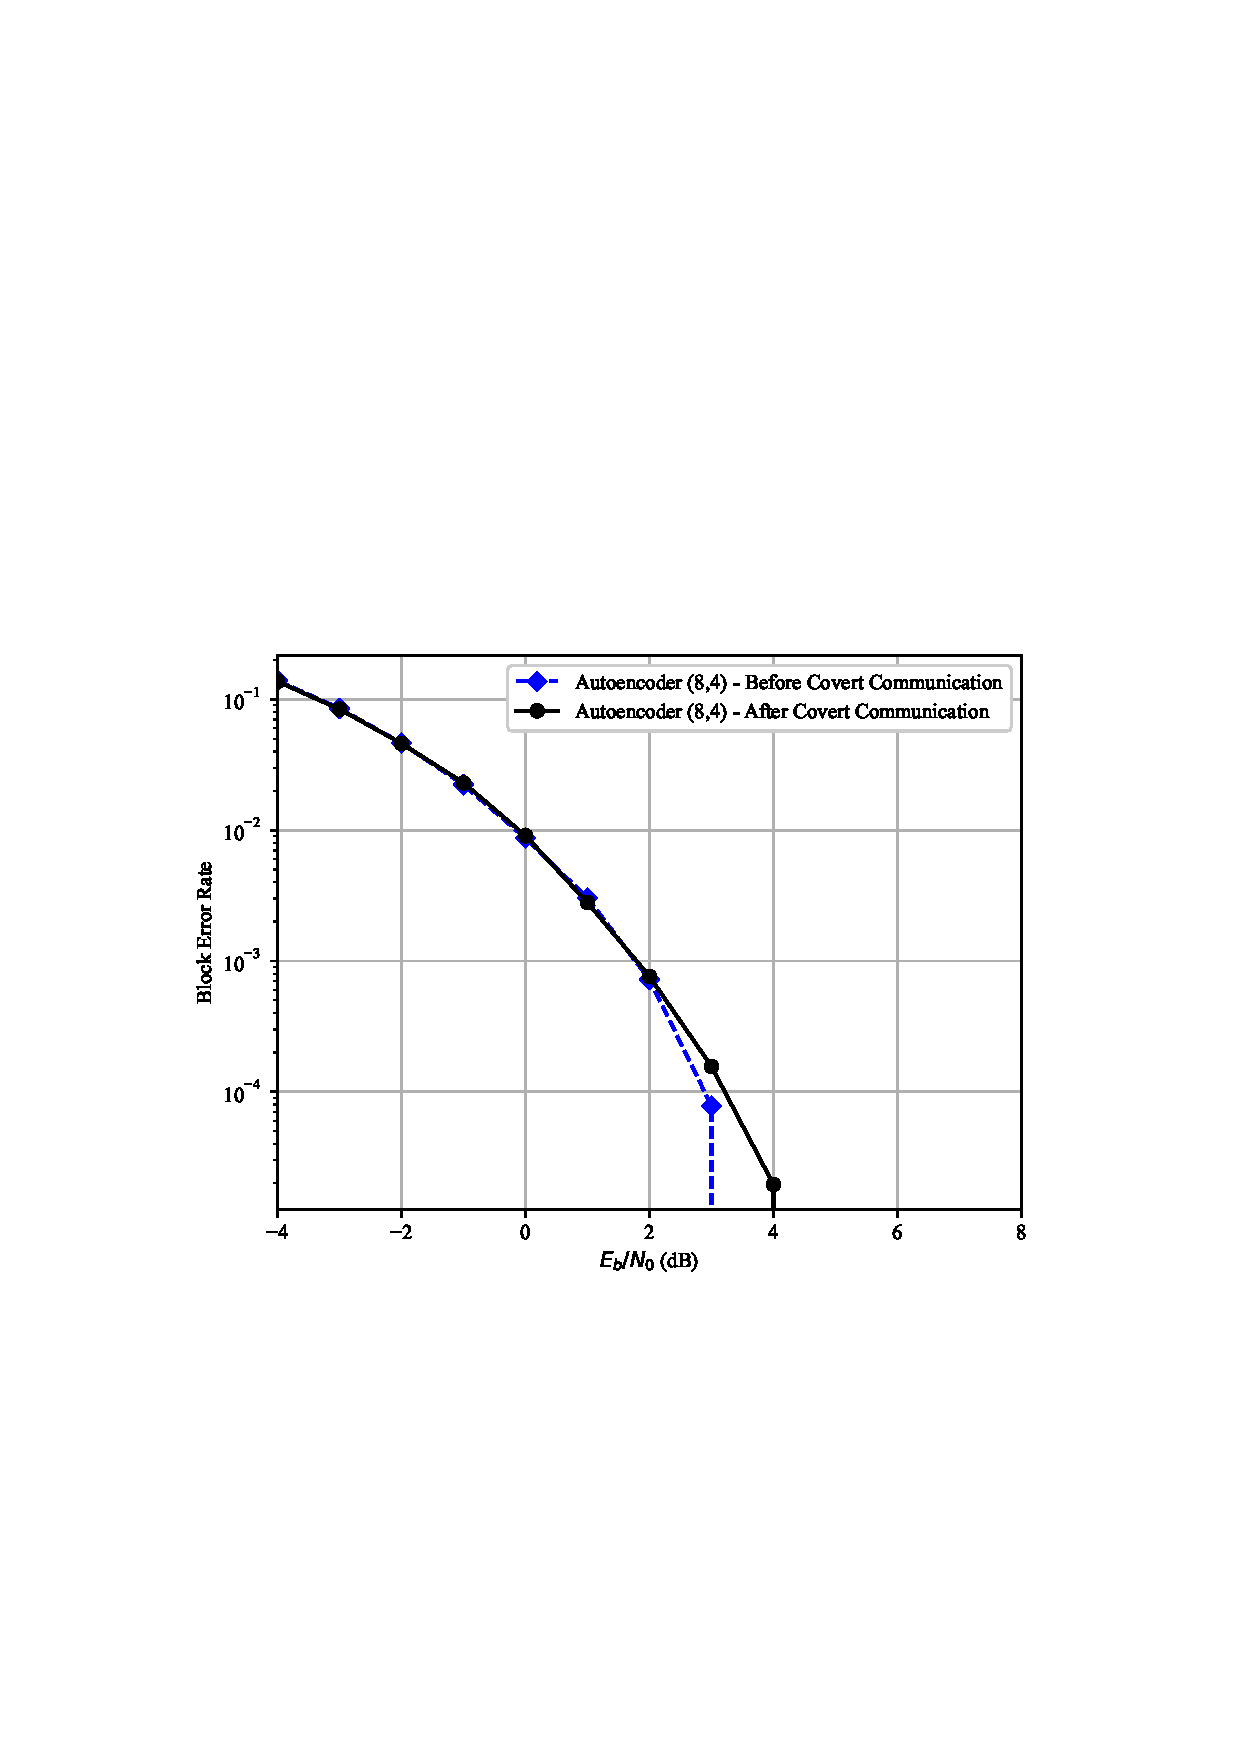
\includegraphics[width=\linewidth]{figs/covert_autoencoder_bler_awgn}
		\caption{Autoencoder's BLER}
		\label{fig:awgn_resutls_ae}
	\end{subfigure}
	\hspace*{\fill}
	\begin{subfigure}{0.28\textwidth}
		\includegraphics[width=\linewidth]{figs/bob_bler_awgn}
		\caption{Bob's BLER}	
		\label{fig:awgn_resutls_bob}
	\end{subfigure}
	\hspace*{\fill}
	\begin{subfigure}{0.28\textwidth}
		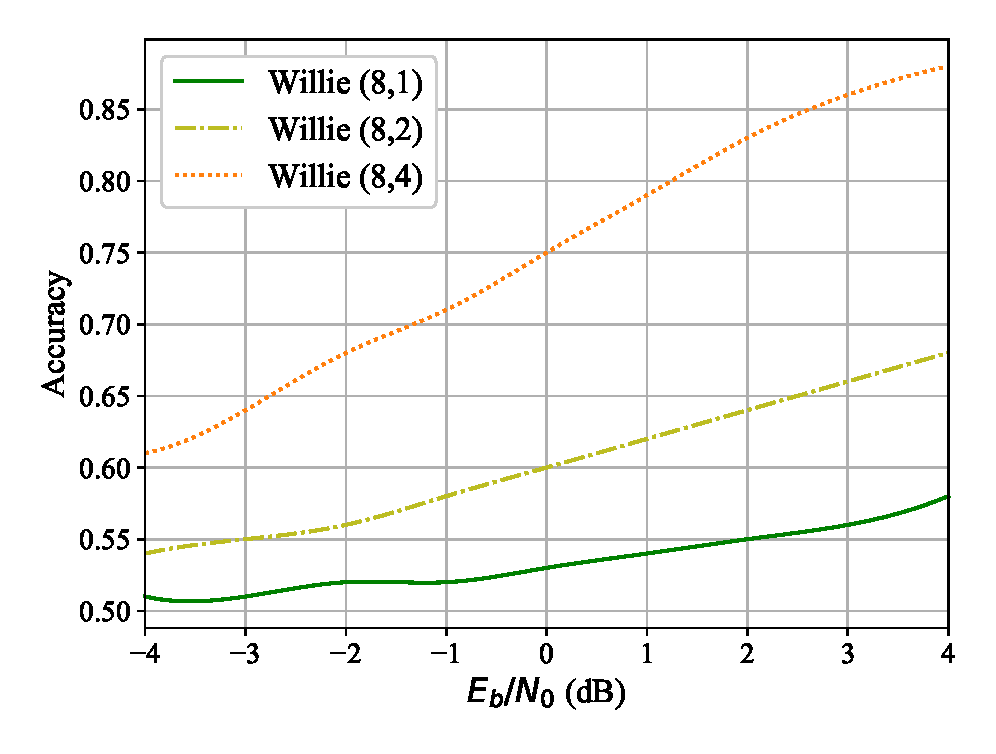
\includegraphics[width=\linewidth]{figs/willie_accuracy_awgn}
		\caption{Willie's accuracy}	
		\label{fig:awgn_resutls_willie}
	\end{subfigure}
	\caption{Trained covert models' performance over AWGN channel for different covert data rates on a range of SNR values.}
	\label{fig:awgn_results}
\end{figure*}
\begin{figure*}[tp!]
	\begin{subfigure}{0.28\textwidth}
		\includegraphics[width=\linewidth]{figs/covert_autoencoder_bler_rayleigh}
		\caption{Autoencoder's BLER}
		\label{fig:rayleigh_resutls_ae}
	\end{subfigure}
	\hspace*{\fill}
	\begin{subfigure}{0.28\textwidth}
		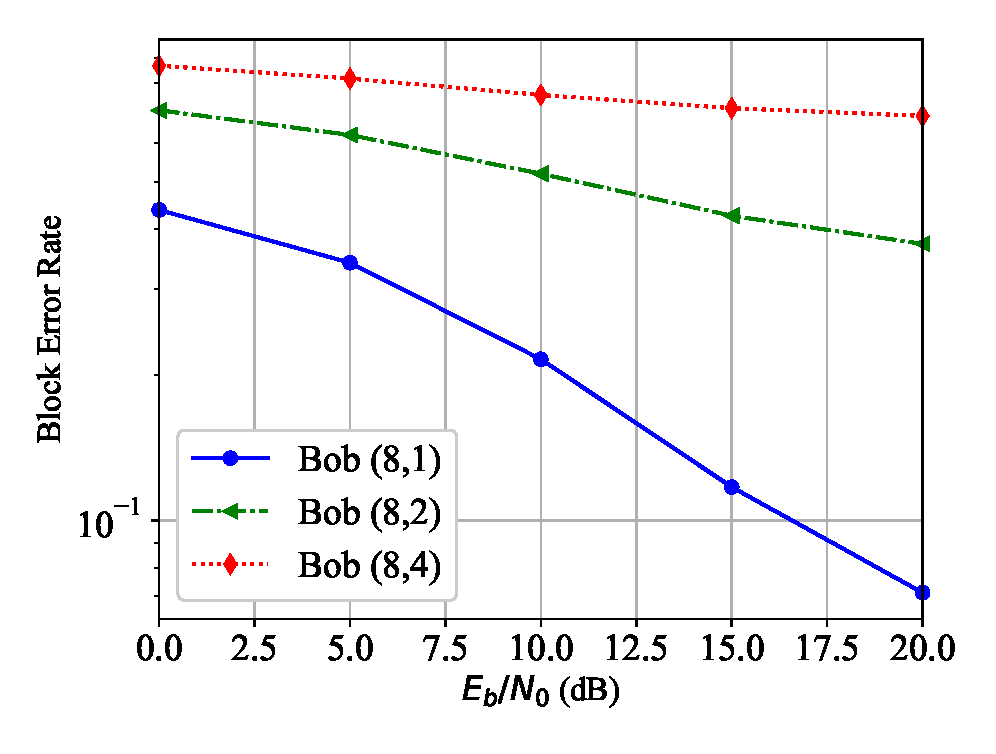
\includegraphics[width=\linewidth]{figs/bob_bler_rayleigh}
		\caption{Bob's BLER}
		\label{fig:rayleigh_resutls_bob}	
	\end{subfigure}
	\hspace*{\fill}
	\begin{subfigure}{0.28\textwidth}
		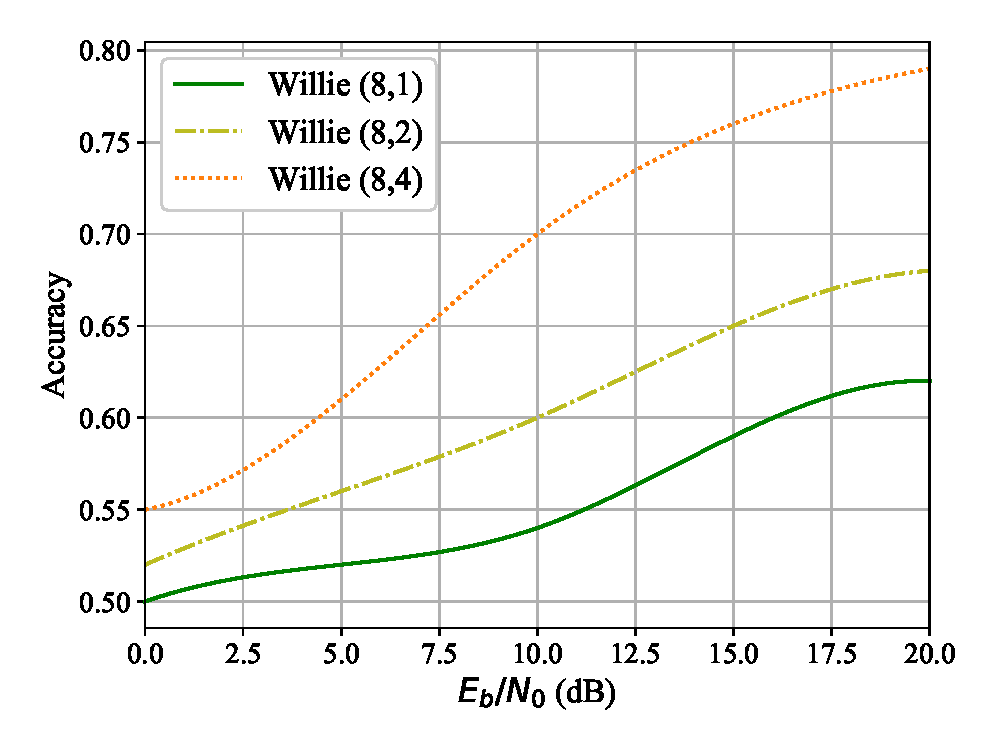
\includegraphics[width=\linewidth]{figs/willie_accuracy_rayleigh}
		\caption{Willie's accuracy}
		\label{fig:rayleigh_resutls_willie}
	\end{subfigure}
	\caption{Trained covert models' performance over Rayleigh fading channel for different covert data rates on a range of SNR values.}
	\label{fig:rayleigh_resutls}
\end{figure*}
\begin{figure*}[tp!]
	\begin{subfigure}{0.28\textwidth}
		\includegraphics[width=\linewidth]{figs/covert_autoencoder_bler_rician}
		\caption{Autoencoder's BLER}
		\label{fig:rician_resutls_ae}
	\end{subfigure}
	\hspace*{\fill}
	\begin{subfigure}{0.28\textwidth}
		\includegraphics[width=\linewidth]{figs/bob_bler_rician}
		\caption{Bob's BLER}
		\label{fig:rician_resutls_bob}	
	\end{subfigure}
	\hspace*{\fill}
	\begin{subfigure}{0.28\textwidth}
		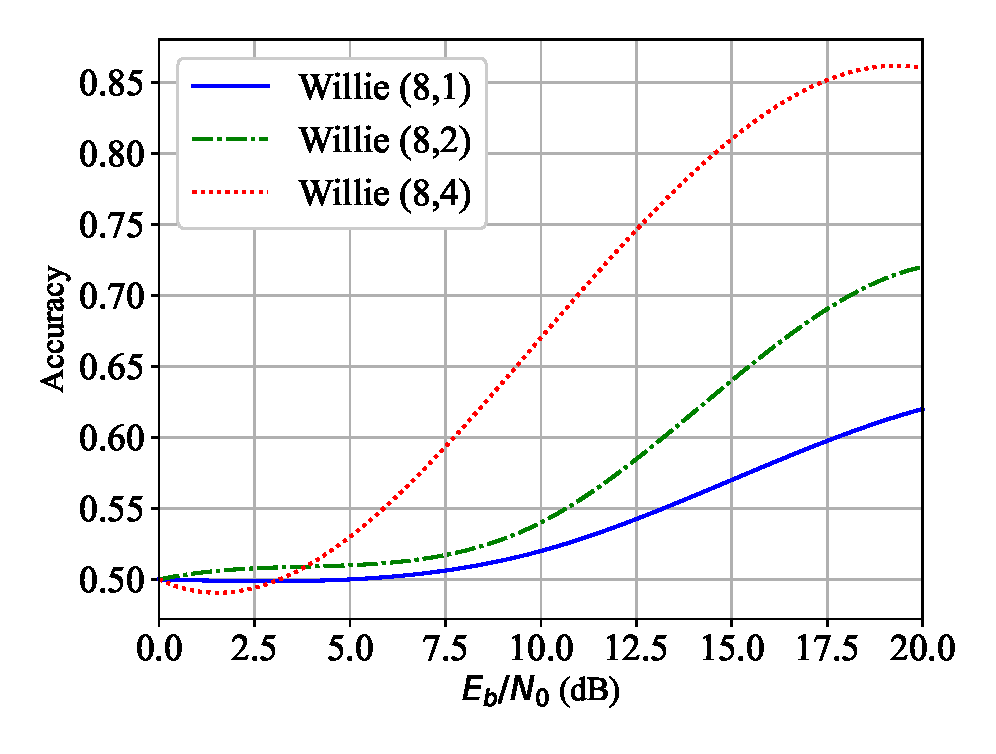
\includegraphics[width=\linewidth]{figs/willie_accuracy_rician}
		\caption{Willie's accuracy}
		\label{fig:rician_resutls_willie}
	\end{subfigure}
	\caption{Trained covert models' performance over Rician fading channel for different covert data rates on a range of SNR values.}
	\label{fig:rician_resutls}
\end{figure*}

\subsection{Covert Model Evaluation Results}
We evaluated the performance of our covert communication models on three different channel models: AWGN, Rayleigh fading, and Rician fading. We used the same training procedure for all settings, but the network architecture of our covert and autoencoder models in the multi-user system differed slightly from that in the single-user setting. Table \ref{table:covert_models_structure} shows these differences.

Since each covert message \(m\) has to be paired with a normal message \(s\), we created the covert model's training and testing sets to have the same number of samples as the autoencoder's. All models were trained for 5000 epochs using the Adam optimizer in an adversarial training setting. We adjusted the importance of each of Alice's objectives by setting \(\lambda_{\mathcal{W}} = 2 \lambda_{\mathcal{B}} = 4 \lambda_{\mathcal{U}}\) for the single-user system, and \(\lambda_{\mathcal{W}} = 3 \lambda_{\mathcal{B}} = 6 \lambda_{\mathcal{U}}\) for the multi-user system in (\ref{alice_loss}). We arrived at these numbers by running a grid search on these parameters. However, our solution is not limited to these parameters, and one can use a different set of parameters to emphasize one specific objective more than the others. In both the single-user and multi-user systems, we started the training with a learning rate of 0.001 for the first 2500 epochs and then made the learning rate ten times smaller for the remaining 2500 epochs. In each epoch, we first updated the parameters of Willie's network using (\ref{willie_loss}), then trained Alice's network for one step using (\ref{alice_loss}), and finally optimized Bob's network based on (\ref{bob_loss}). Although we trained our autoencoder network on a fixed SNR value, we found that our covert scheme performed better when trained on a range of SNR values. We achieved this by randomly switching the SNR value within a predetermined range after each epoch of training. Training our models this way not only helped Alice better preserve the normal communication's accuracy but also enabled Bob to decode covert messages more accurately on lower SNR values. Accordingly, we started by setting the training SNR to the value that the autoencoder was trained on and incrementally expanded the SNR range from both ends until no further improvement was observed. As a result, in the single-user system, we settled on the range of -2dB to 8 dB for the AWGN channel and 10dB to 30dB for both the Rayleigh and Rician fading channels. In the multi-user system, the optimal range was found within the 0dB to 10dB range for the AWGN channel, 0dB to 20dB for the Rician channel, and 10dB to 30dB for the Rayleigh channel.

\begin{figure*}[tp!]
	\begin{subfigure}{0.28\textwidth}
		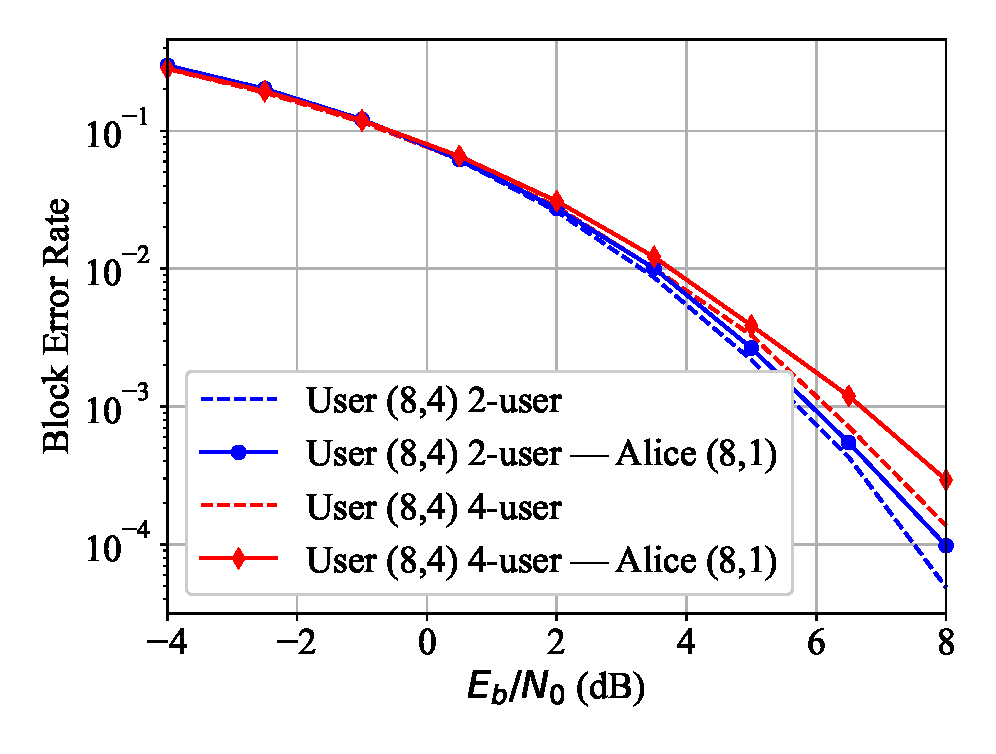
\includegraphics[width=\linewidth]{figs/multi_covert_autoencoder_bler_awgn}
		\caption{Autoencoder's BLER}
		\label{fig:multi_awgn_results_ae}
	\end{subfigure}
	\hspace*{\fill}
	\begin{subfigure}{0.28\textwidth}
		\includegraphics[width=\linewidth]{figs/multi_bob_bler_awgn}
		\caption{Bob's BLER}	
		\label{fig:multi_awgn_results_bob}
	\end{subfigure}
	\hspace*{\fill}
	\begin{subfigure}{0.28\textwidth}
		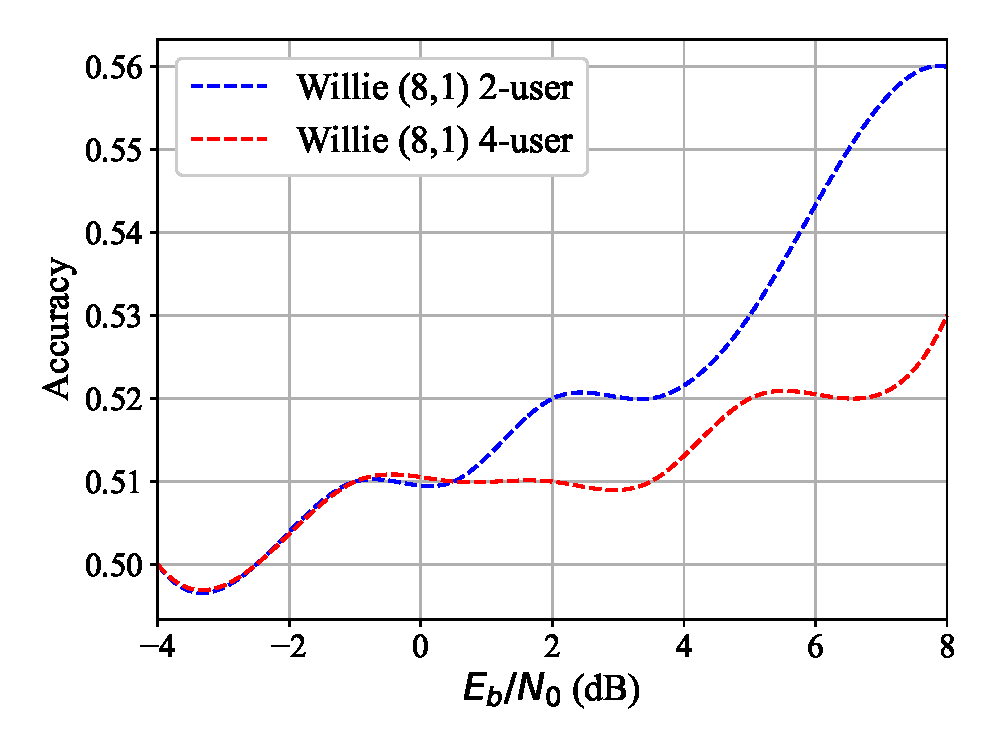
\includegraphics[width=\linewidth]{figs/multi_willie_accuracy_awgn}
		\caption{Willie's accuracy}	
		\label{fig:multi_awgn_results_willie}
	\end{subfigure}
	\caption{Trained covert models' performances over AWGN channel for systems with different numbers of users across a range of SNR values.}
	\label{fig:multi_awgn_results}
\end{figure*}
\begin{figure*}[tp!]
	\begin{subfigure}{0.28\textwidth}
		\includegraphics[width=\linewidth]{figs/multi_covert_autoencoder_bler_rayleigh}
		\caption{Autoencoder's BLER}
		\label{fig:multi_rayleigh_results_ae}
	\end{subfigure}
	\hspace*{\fill}
	\begin{subfigure}{0.28\textwidth}
		\includegraphics[width=\linewidth]{figs/multi_bob_bler_rayleigh}
		\caption{Bob's BLER}
		\label{fig:multi_rayleigh_results_bob}	
	\end{subfigure}
	\hspace*{\fill}
	\begin{subfigure}{0.28\textwidth}
		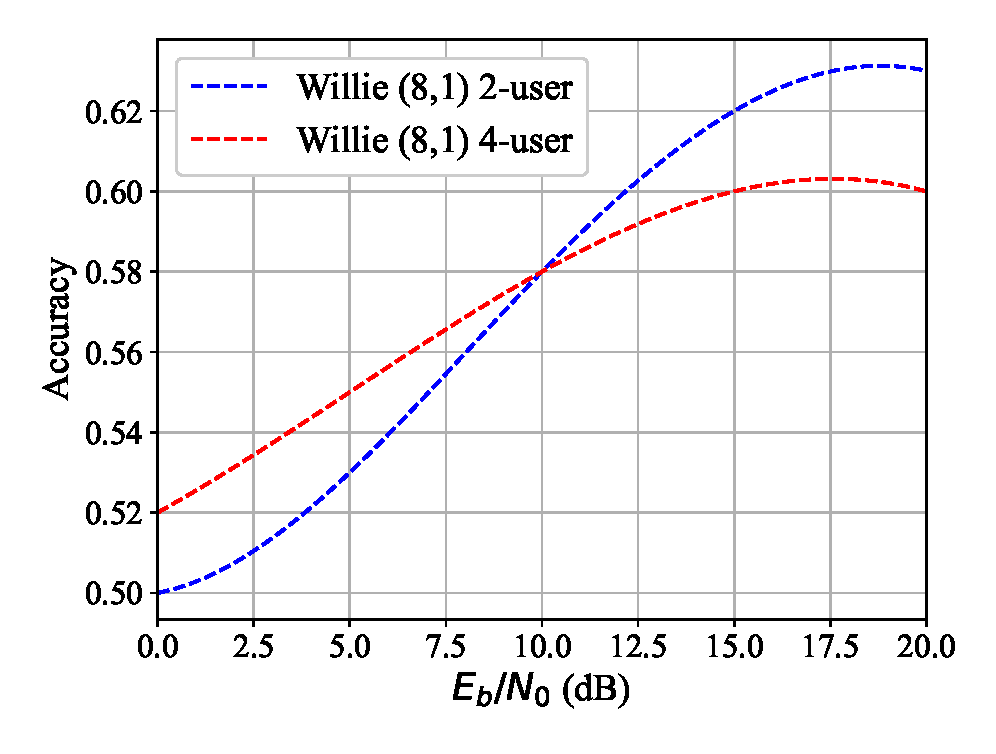
\includegraphics[width=\linewidth]{figs/multi_willie_accuracy_rayleigh}
		\caption{Willie's accuracy}
		\label{fig:multi_rayleigh_results_willie}
	\end{subfigure}
	\caption{Trained covert models' performances over Rayleigh channel for systems with different number of users across a range of SNR values.}
	\label{fig:multi_rayleigh_results}
\end{figure*}
\begin{figure*}[tp!]
	\begin{subfigure}{0.28\textwidth}
		\includegraphics[width=\linewidth]{figs/multi_covert_autoencoder_bler_rician}
		\caption{Autoencoder's BLER}
		\label{fig:multi_rician_results_ae}
	\end{subfigure}
	\hspace*{\fill}
	\begin{subfigure}{0.28\textwidth}
		\includegraphics[width=\linewidth]{figs/multi_bob_bler_rician}
		\caption{Bob's BLER}
		\label{fig:multi_rician_results_bob}	
	\end{subfigure}
	\hspace*{\fill}
	\begin{subfigure}{0.28\textwidth}
		\includegraphics[width=\linewidth]{figs/multi_willie_accuracy_rician}
		\caption{Willie's accuracy}
		\label{fig:multi_rician_results_willie}
	\end{subfigure}
	\caption{Trained covert models' performances over Rician channel for systems with different number of users across a range of SNR values.}
	\label{fig:multi_rician_results}
\end{figure*}

We started our experiments with single-user models. First, we evaluated our covert models by sending 1 bit of covert data over 8 channel uses and then gradually increased the number of covert bits to see how increasing the covert data rate affected each component of our covert scheme. We used the notations \(Alice (n,k)\), \(Bob (n,k)\), and \(Willlie (n,k)\) to differentiate models with different covert data rates, and their interpretation was the same as that of the autoencoder model.

After evaluating the reliability of our covert models for different covert data rates, we now aim to measure the robustness of our covert scheme against the number of users in multi-user systems. To do this, we evaluate our covert models in systems comprising of 2 and 4 users. This will help us understand how adding users to the system affects our covert models' performance and whether this has a greater impact on communication than increasing the covert data rate.

\textbf{Training Procedure}: Figure \ref{fig:traning_progress} shows the progress of each covert actor's accuracy on the test set during the training process for both single-user and multi-user systems. As the training progresses, Bob gradually learns to decode covert messages \(m\) and establishes reliable communication with Alice. After a few epochs as the covert communication begins to take form and stabilize, the signals start to deviate from their original distribution, which helps Willie to better detect covert signals. When Willie's accuracy increases, the term \(\mathcal{L}_{\mathcal{W}}\) dominates the other two objectives of Alice's loss function in (\ref{alice_loss}). As a result, Alice gradually sacrifices accuracy for undetectability. Soon after, the training process reaches a stable point where neither of the covert models sees any significant improvement in accuracy as the training progresses. At the end of the training, \textbf{the Users' accuracy remains intact, Bob achieves reliable covert communication accuracy, and Willie stabilizes at around 50$\sim$60\% accuracy, which, for a binary classifier, is very close to random guessing accuracy.}

\textbf{Covert Data Rate}: Figures \ref{fig:awgn_results}, \ref{fig:rayleigh_resutls}, and \ref{fig:rician_resutls} illustrate the performance of our scheme for different covert data rates and how reliable our covert models are at different covert data rates. As we expected, with increasing covert data rates, covert communication becomes more unreliable, its impact on the normal communication increases, and detection becomes easier for the observer. These plots indicate that sending covert data at high rates makes covert communication unreliable. Therefore, we proceed with the lowest covert data rate, which involves sending 1 bit of data over 8 channel uses, to evaluate our models in multi-user systems.

\textbf{Number of Users}: Figures \ref{fig:multi_awgn_results}, \ref{fig:multi_rayleigh_results}, and \ref{fig:multi_rician_results} present our final results for 2-user and 4-user systems, demonstrating how the number of users in the system affects our model's performance. For the AWGN channel, we can observe that adding more users does not change the model's overall performance in both cases. Furthermore, as the number of users increases, there is almost no impact on the normal receivers from the covert transmissions, and Bob and Willie's performances remain almost the same. However, for the Rayleigh and Rician channels, we can observe a degree of freedom effect, where an increasing number of users makes it more challenging for the covert users to avoid interfering with the ongoing normal communication. Unlike the AWGN channel, adding more users in these cases degrades Bob's performance and improves Willie's detection ability.
\begin{figure}[tp!]
	\center
	\begin{subfigure}{0.24\textwidth}
		\includegraphics[width=\linewidth]{figs/training_progress}
		\caption{Single-user system}	
	\end{subfigure}
	\begin{subfigure}{0.24\textwidth}
		\includegraphics[width=\linewidth]{figs/multi_training_progress}
		\caption{Multi-user system}	
	\end{subfigure}
	\caption{Evaluation results of our covert and autoencoder models during the training process show the system reaches a stable point after successful training.}
	\label{fig:traning_progress}
\end{figure}

\textbf{Undetectability}: Willie's detection accuracy in percentage can be found in Figures \ref{fig:awgn_resutls_willie}, \ref{fig:rayleigh_resutls_willie}, and \ref{fig:rician_resutls_willie} for single-user systems, and in Figures \ref{fig:multi_awgn_results_willie}, \ref{fig:multi_rayleigh_results_willie}, \ref{fig:multi_rician_results_willie} for multi-user systems. His detection performance is evaluated over a range of SNR values for detecting signals as covert and normal. These plots give us an intuition on how likely our covert signals are to be detected by a target system's observer for different covert rates at each SNR value.
Overall, we observe that increasing the covert data rate makes the covert channel more exposed than having multiple users in the system. It is observed that Willie's detection accuracy increases for every added single bit of covert data, while his accuracy is roughly unaffected by the presence of more users in the system.

\begin{figure}[bp!]
	\begin{subfigure}{0.24\textwidth}
		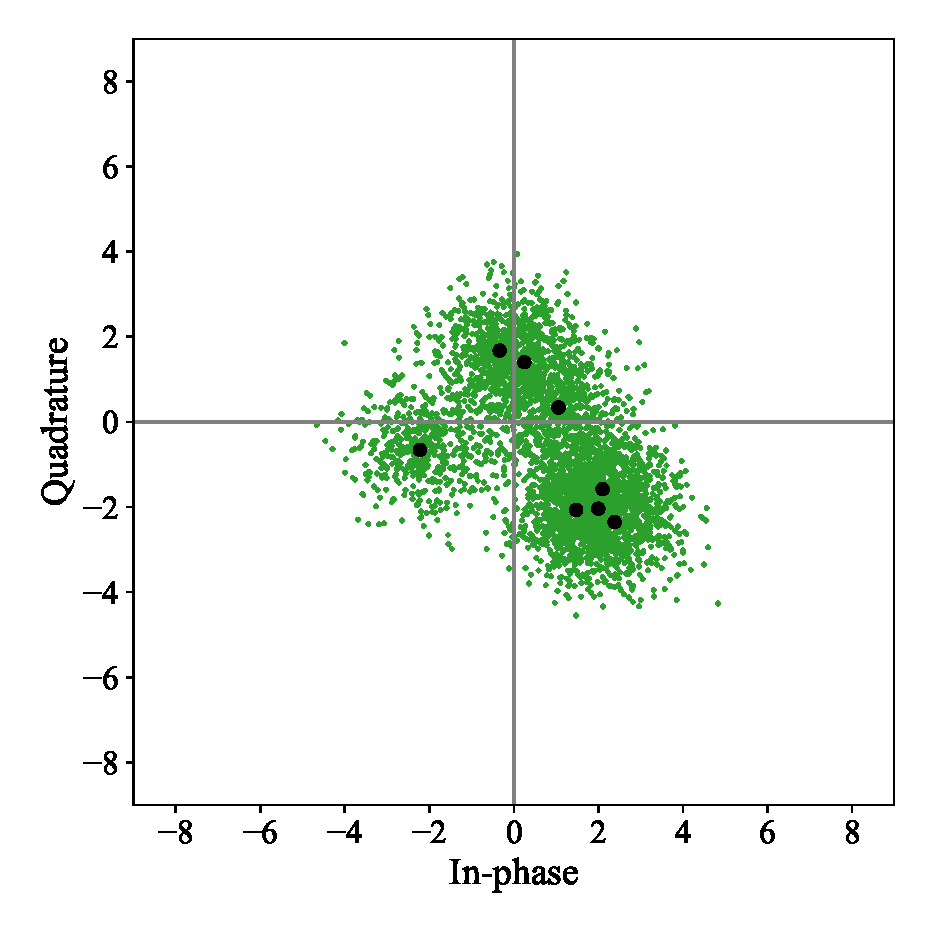
\includegraphics[width=\linewidth]{figs/awgn_normal_constellation}
		\caption{Without covert transmission}
	\end{subfigure}
	\hfill
	\begin{subfigure}{0.24\textwidth}
		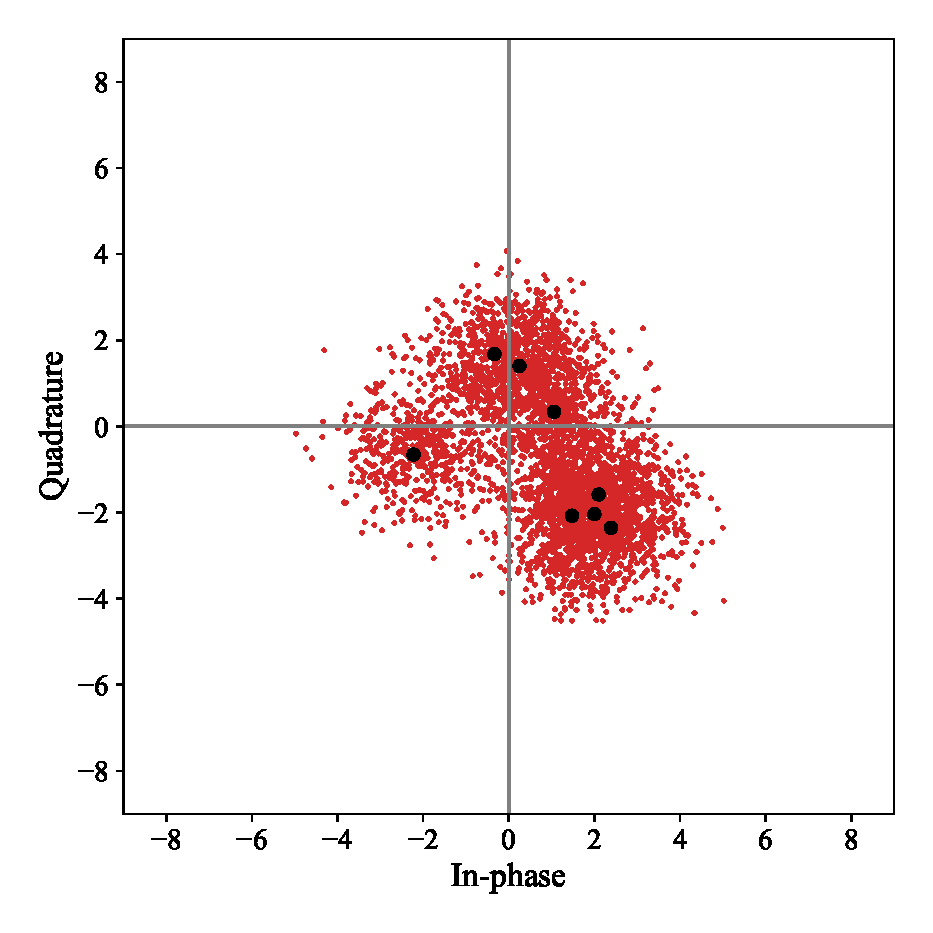
\includegraphics[width=\linewidth]{figs/awgn_covert_constellation}
		\caption{With covert transmission}	
	\end{subfigure}
	\caption{Comparing AWGN channel constellation clouds of a signal before and after our covert scheme being applied.}
	\label{fig:awgn_constellation}
\end{figure}
\begin{figure}[tp!]
	\begin{subfigure}{0.24\textwidth}
		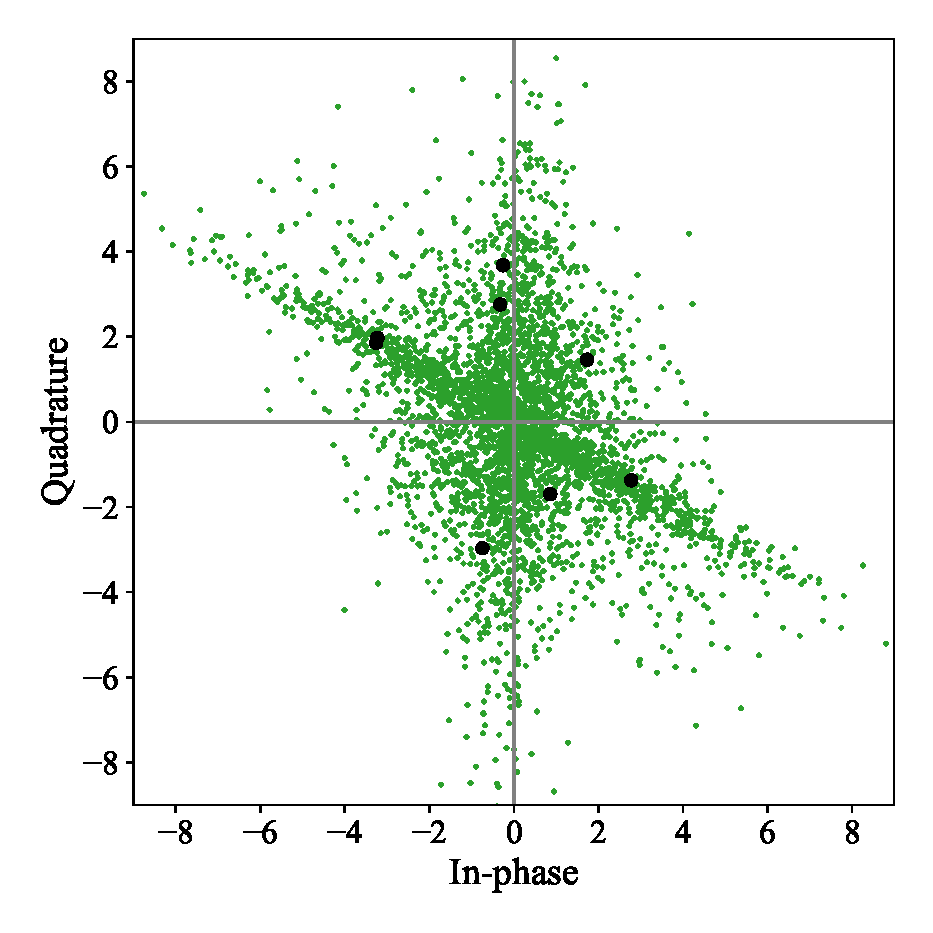
\includegraphics[width=\linewidth]{figs/rayleigh_normal_constellation}
		\caption{Without covert transmission}
	\end{subfigure}
	\hfill
	\begin{subfigure}{0.24\textwidth}
		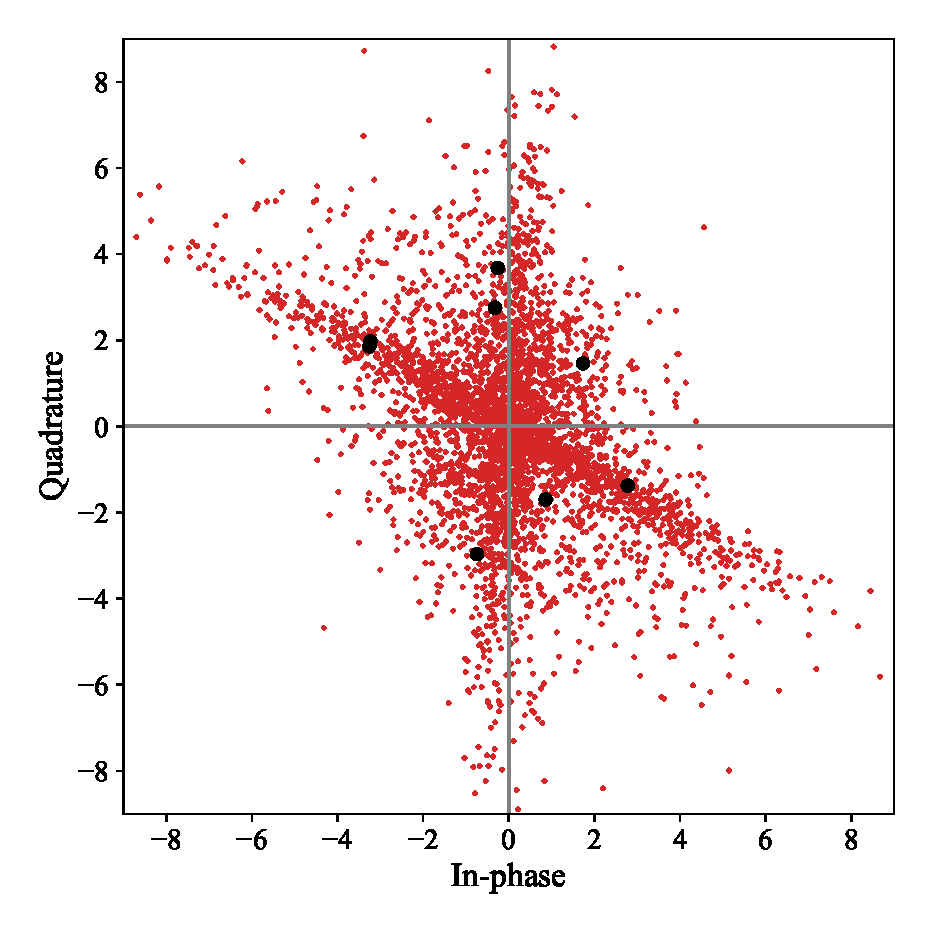
\includegraphics[width=\linewidth]{figs/rayleigh_covert_constellation}
		\caption{With covert transmission}	
	\end{subfigure}
	\caption{Comparing Rayleigh fading channel constellation clouds of a signal before and after our covert scheme being applied.}
	\label{fig:rayleigh_constellation}
\end{figure}
\begin{figure}[tp!]
	\begin{subfigure}{0.24\textwidth}
		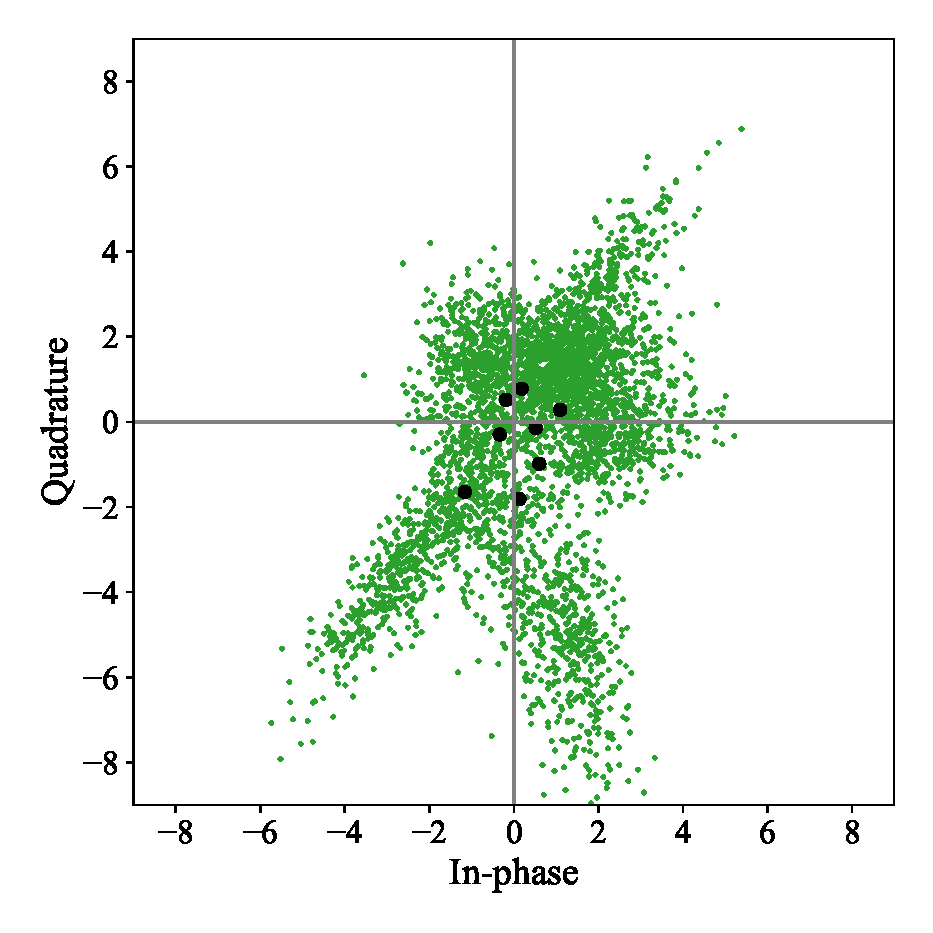
\includegraphics[width=\linewidth]{figs/rician_normal_constellation}
		\caption{Without covert transmission}
	\end{subfigure}
	\hfill
	\begin{subfigure}{0.24\textwidth}
		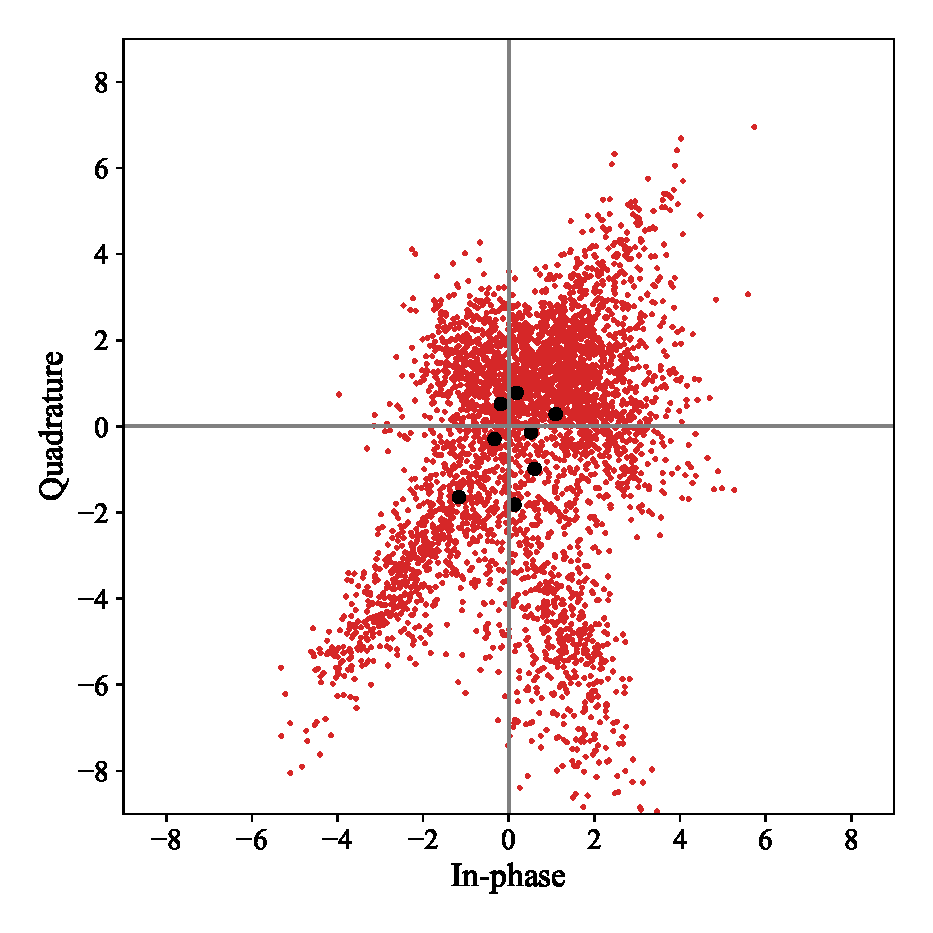
\includegraphics[width=\linewidth]{figs/rician_covert_constellation}
		\caption{With covert transmission}	
	\end{subfigure}
	\caption{Comparing Rician fading channel constellation clouds of a signal before and after our covert scheme being applied.}
	\label{fig:rician_constellation}
\end{figure}

Figures \ref{fig:awgn_constellation}, \ref{fig:rayleigh_constellation}, and \ref{fig:rician_constellation} compare the constellation clouds of covert and normal signals for AWGN, Rayleigh, and Rician fading channels in the single-user system. We marked each symbol of the encoder's output signal as black circle points on the constellation diagrams. The red constellation cloud shows how covert signals scatter after passing through the channel, and the green cloud shows this for normal signals. Since data is sent over 8 channel uses, there are 8 black points on the chart. To maintain consistency with Willie's accuracy and Bob's error rate for all channel models, we set the SNR value to 6dB for the AWGN, 15dB for the Rayleigh fading channel, and 16dB for the Rician fading channel. This ensured that, in all channel models, the probability of detection remained relatively the same, and the covert communication BLER stayed below \(10^{-1}\). This area of operation provided Alice and Bob relative reliability in their covert communication while maintaining their covertness.
Looking at these figures, the signal constellation diagrams before and after applying our covert model are very similar, showing that Alice has perfectly learned to cloak the covert signals into the distribution of the channel's noise.